% Generated by scripts/build_manuscript.py from sections/witness_experiments.tex.
% Edit the source, then regenerate; all outcomes are retained.
\section{Lower-bound comparisons beyond two atoms}
\label{sec:witness-comparison}

The two-atom law in Proposition~\ref{main-prop:two-atom} has an exact population
witness. To distinguish a loose population bound from finite-sample uncertainty,
we evaluate eight finite-support distributions (Table~\ref{tab:witness-laws}).
They include deterministic and noisy targets, histories assigned identical
features despite different targets, rare conflicting targets, and a case in
which affine decoders are less expressive than general Lipschitz decoders.
For every method, $R^*$ is the minimum MSE over the same full scalar
$1$-Lipschitz class with outputs in $[-1,1]$. These explicit representations
isolate the behavior of the certificates;
they do not measure the forecasting accuracy of learned KAHM features.

\begin{table}[t]
\centering\footnotesize
\setlength{\tabcolsep}{3pt}
\begin{tabular}{llll}
\toprule
Law & Representation values $u_i$ & Targets $y_i$ & Stratum labels $c(u_i)$ \\
\midrule
Collapsed binary & $(0,0)$ & $(-1,1)$ & $(0,0)$ \\
Two atoms & $(-.6/\sqrt2,.6/\sqrt2)$ & $(-1,1)$ & $(0,0)$ \\
Three-point V & $(-1,0,1)$ & $(1,-1,1)$ & $(0,0,1)$ \\
Five-point zigzag & $(-1,-.5,0,.5,1)$ & $(-1,1,-1,1,-1)$ & $(0,0,1,1,1)$ \\
Partial collapse & $(-1,-1,0,0,1,1)$ & $(-1,.2,-.2,.2,-.2,1)$ & $(0,0,1,1,2,2)$ \\
Noisy affine & $(-1,-1,0,0,1,1)$ & $(-1,0,-.5,.5,0,1)$ & $(0,0,1,1,2,2)$ \\
Rare conflict & $(3,0,1)$ & $(0,-1,1)$ & $(0,1,1)$ \\
Affine mismatch & $(-1,0,1)$ & $(-.5,.5,-.5)$ & $(0,0,0)$ \\
\bottomrule
\end{tabular}
\caption{Prespecified joint supports for the lower-bound comparison. Entry $i$ gives one possible pair $(U,Y)=(u_i,y_i)$. Each row assigns equal probabilities to its entries, except rare conflict, whose probabilities are $(.9,.05,.05)$. Repeated representation values retain different possible targets. Stratum labels depend only on $U$ and are fixed before calibration. Every law uses $|u-u'|$, $\kappa=1$, and predictions in $[-1,1]$.}
\label{tab:witness-laws}
\end{table}


\paragraph{Protocol and comparators.}
The protocol was recorded before sampling. Each law uses 300 independent
calibration samples at each $n\in\{64,256,1024,4096\}$, totaling 9,600 trials.
The four primary methods share each sample and each receive a separate
one-sided failure probability $0.05$; no joint $95\%$ event across methods
is asserted. We compare the disjoint-pair empirical Bernstein (EB) bound in
Theorem~\ref{main-thm:episode-certificate}, the range-aware centered bound in
Appendix~\ref{main-app:centered-range-aware}, the dual-certified empirical risk
minimization (ERM) bound with Kullback--Leibler (KL) correction in
\eqref{main-eq:erm-kl-lower}, and the
stratified certificate in Theorem~\ref{main-thm:stratified-certificate}.
The primary stratified method estimates the stratum probabilities from the
calibration data. Both primary pairwise methods use the generic score range
$[0,2]$, obtained from a target diameter of two.
Prespecified secondary analyses tighten this range using the known support,
use known stratum masses, or replace the empirical-minimum correction by
Hoeffding's bound. The result archive includes every secondary analysis.

The empirical and population optimization programs use the full Lipschitz
class, with global extension from the finite support. Feasible primal and dual
values bracket each optimum; the largest empirical gap is
$4.01\times10^{-11}$. Analytic checks cover all eight population optima.
An unprojected affine optimum is never used as a Lipschitz lower bound: in the
mismatch law, the former is $2/9$ and the latter is zero.

\begin{table}[t]
\centering\small
\setlength{\tabcolsep}{3pt}
\begin{tabular}{lrrrrrrrr}
\toprule
& \multicolumn{4}{c}{Population quantities} & \multicolumn{4}{c}{Mean lower endpoint, $n=4096$} \\
\cmidrule(lr){2-5}\cmidrule(lr){6-9}
Law & $R^*$ & $W$ & $W_{\rm str}$ & $C$ & Pair & Centered & ERM & Strat. \\
\midrule
Collapsed binary & 1.0000 & 1.0000 & 1.0000 & 1.0000 & 0.9306 & 0.9149 & 0.9345 & 0.9237 \\
Two atoms & 0.3315 & 0.3315 & 0.3315 & 0.3315 & 0.3034 & 0.2807 & 0.2908 & 0.3001 \\
Three-point V & 0.2222 & 0.2222 & 0.1667 & 0.0160 & 0.1996 & 0.0000 & 0.1890 & 0.1355 \\
Five-point zigzag & 0.5400 & 0.3800 & 0.5250 & 0.0744 & 0.3408 & 0.0186 & 0.4891 & 0.4442 \\
Partial collapse & 0.2533 & 0.0867 & 0.2533 & 0.0000 & 0.0646 & 0.0000 & 0.2178 & 0.1772 \\
Noisy affine & 0.2500 & 0.0972 & 0.2500 & 0.0000 & 0.0777 & 0.0000 & 0.2145 & 0.1801 \\
Rare conflict & 0.0250 & 0.0025 & 0.0250 & 0.0000 & 0.0000 & 0.0000 & 0.0148 & 0.0059 \\
Affine mismatch & 0.0000 & 0.0000 & 0.0000 & 0.0000 & 0.0000 & 0.0000 & 0.0000 & 0.0000 \\
\bottomrule
\end{tabular}
\caption{Finite-support comparison on the same full scalar Lipschitz class. $R^*$ is the minimum MSE, $W$ the unconditional pair witness, $W_{\rm str}$ the prespecified stratified witness, and $C$ the centered population bound. The last four columns average 300 independent calibration samples. Each method separately has nominal one-sided confidence $95\%$; no joint confidence across columns is asserted. Empirical risk minimization (ERM) uses a dual-certified empirical minimum and bounded-loss Kullback--Leibler (KL) inversion. Primary stratification estimates the stratum masses. All quantities are in MSE units.}
\label{tab:witness-comparison}
\end{table}


\paragraph{Population slack and finite-sample cost.}
Table~\ref{tab:witness-comparison} reports population quantities separately
from mean calibrated endpoints. On partial collapse, stratification raises
the population witness from $0.0867$ to the exact minimum $0.2533$.
At $n=4096$, its mean endpoint is $0.1772$, compared with $0.0646$ for
unconditional pairing and $0.2178$ for empirical minimization. Stratification
also improves the five-point and noisy-affine witnesses. It worsens the
three-point witness, from $0.2222$ to $0.1667$, demonstrating that a fixed
partition need not help.

Empirical minimization gives the largest mean endpoint on most richer laws;
the pair bound is larger on the partially separated two-atom and three-point
laws at $n=4096$. Accounting for a known representation range substantially
improves centered calibration when the representation is constant.
The two-atom comparison in Section~\ref{sec:experiments}
quantifies how treating a known zero variance as unknown can weaken a centered
endpoint. Consequently, the relative performance of pairwise and centered
certificates depends on the estimator and the structural information supplied
to it.

\begin{figure}[p]
\centering
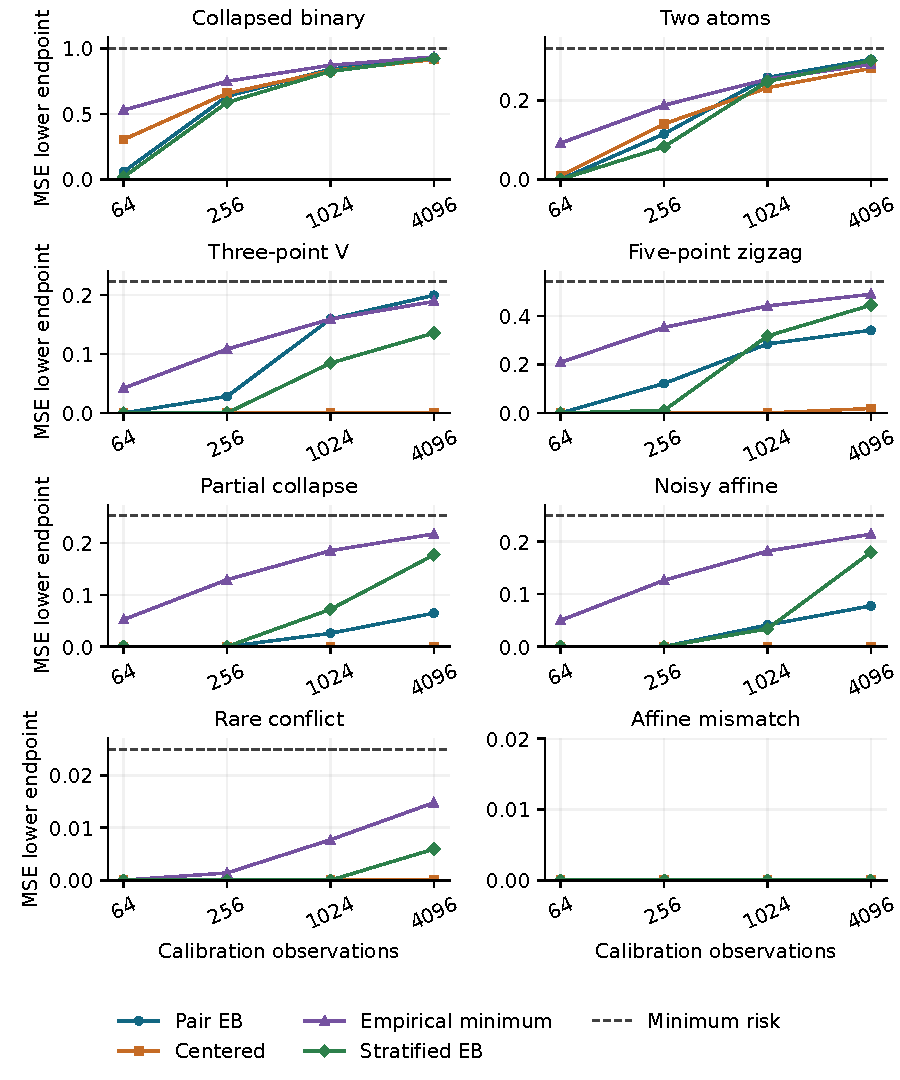
\includegraphics[width=\linewidth]{figures/witness_sample_size.pdf}
\caption{Mean lower endpoints over all 300 repetitions at each calibration
size for every prespecified law. Dashed lines show minimum population MSE.
Each method has its own $95\%$ one-sided confidence statement. The result
archive provides endpoint quantiles, Monte Carlo confidence
intervals, secondary methods, and all individual trials.}
\label{fig:witness-sample-size}
\end{figure}

\paragraph{Positive tolerances, coverage, and computation.}
The fixed RMSE tolerances are $0.10$, $0.25$, and $0.50$ for every law.
On partial collapse at $n=4096$, unconditional pairing excludes tolerance
$0.25$ in 211 of 300 trials; empirical minimization and primary stratification
both exclude it in all 300. Rare conflicts remain difficult: their exact
risk is $0.025$, but unconditional pairing and primary stratification never
exclude tolerance $0.10$ at this sample size. Empirical minimization excludes
it in all 300 trials. Tightening the stratified score range using the known
support raises its exclusion count to 284; additionally supplying known masses
raises it to 300. The gain therefore depends on both pairing and available
information.

All four primary methods have zero observed coverage violations across the
prespecified grid. This simulation does not prove coverage; each law--size
cell has only 300 repetitions, and the result archive gives binomial Monte
Carlo confidence intervals. At $n=4096$, medians across the eight
law-wise median computation times are $31.3$, $34.7$, $265.4$, and $165.0$
$\mu$s for pair EB, centered, empirical minimum, and stratified EB,
respectively. These single-machine measurements use a precomputed finite-support
pair-score table and include sample statistics, confidence corrections, and
ERM optimization after representation lookup. They exclude feature learning
and do not establish a computational advantage on large continuous supports.
The frozen protocol, sufficient statistics, dual certificates, and complete
analysis are in \path{results/witness_comparison}.
